\section{Các mô hình SVM biên mềm (soft-margin SVMs)}

\begin{frame}{Nhắc lại về điểm yếu của Linear SVMs}
  \begin{itemize}
    \item Hard-Margin yêu cầu \textbf{mọi điểm} phải nằm ngoài margin và được phân loại đúng.
    \item Trong thực tế:
      \begin{itemize}
        \item Dữ liệu thường có nhiễu, chồng lấn nhẹ.
        \item Một điểm outlier có thể khiến bài toán \textbf{vô nghiệm}.
        \item Hoặc margin bị ép rất hẹp → overfitting.
      \end{itemize}
  \end{itemize}
  \vspace{0.3cm}
  \centering
  \textbf{→ Cần một mô hình "mềm dẻo" hơn, cho phép một số điểm vi phạm margin.}
\end{frame}

\begin{frame}{Biến lỏng slack $\xi_i$​ và điều kiện lề mềm (soft margin)}
  \begin{columns}
    \begin{column}{0.5\textwidth}
      \begin{itemize}
        \item \textbf{Biên cứng:} $y_i(\bm{w}^T\bm{x}_i + b) \ge 1$ (quá cứng nhắc).
        \item \textbf{Biên mềm:} thêm $\xi_i \ge 0$ để nới lỏng:
        \[
        y_i(\bm{w}^T\bm{x}_i + b) \ge 1 - \xi_i
        \]
        \item $\xi_i$ đo mức độ "vi phạm" của điểm $i$:
        \begin{itemize}
          \item $\xi_i = 0$: điểm an toàn (ngoài margin).
          \item $0 < \xi_i \le 1$: lấn vào margin nhưng vẫn đúng lớp.
          \item $\xi_i > 1$: bị phân loại sai.
        \end{itemize}
      \end{itemize}
    \end{column}
    \begin{column}{0.5\textwidth}
      \centering
      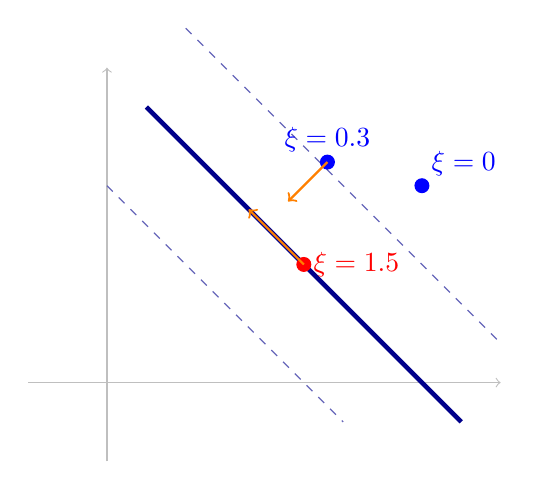
\begin{tikzpicture}[scale=1.0]
        \draw[->, gray!50] (-1,0) -- (5,0);
        \draw[->, gray!50] (0,-1) -- (0,4);
        \draw[ultra thick, DarkBlue] (0.5,3.5) -- (4.5,-0.5);
        \draw[dashed, DarkBlue!60] (0,2.5) -- (3,-0.5);
        \draw[dashed, DarkBlue!60] (1,4.5) -- (5,0.5);
        % Điểm
        \filldraw[blue] (4,2.5) circle (2.5pt) node[above right] {$\xi=0$};
        \filldraw[blue] (2.8,2.8) circle (2.5pt) node[above] {$\xi=0.3$};
        \draw[->, orange, thick] (2.8,2.8) -- (2.3,2.3);
        \filldraw[red] (2.5,1.5) circle (2.5pt) node[right] {$\xi=1.5$};
        \draw[->, orange, thick] (2.5,1.5) -- (1.8,2.2);
      \end{tikzpicture}
    \end{column}
  \end{columns}
\end{frame}

\begin{frame}{Tại sao ràng buộc lại là $y_i(\bm{w}^T\bm{x}_i + b) \ge 1 - \xi_i$?}
  \begin{block}{Gốc rễ: Yêu cầu về khoảng cách trong hard-margin}
    Trong không gian, khoảng cách từ điểm $\bm{x}_i$ đến siêu phẳng là $$\frac{|\bm{w}^T\bm{x}_i + b|}{\|\bm{w}\|}$$. \\
    Để đảm bảo độ rộng \textbf{margin} là $\frac{2}{\|\bm{w}\|}$, mọi điểm phải cách siêu phẳng \textbf{tối thiểu} $\frac{1}{\|\bm{w}\|}$. 
    
    \begin{center}
      Điều kiện đó được viết gọn thành: $y_i(\bm{w}^T\bm{x}_i + b) \ge 1$.
    \end{center}
  \end{block}

\end{frame}

\begin{frame}{Tại sao ràng buộc lại là $y_i(\bm{w}^T\bm{x}_i + b) \ge 1 - \xi_i$?}
    \textbf{Vậy $1 - \xi_i$ là gì?}
    \begin{itemize}
        \item $\xi_i$ là \textbf{khoảng cách vi phạm đã chuẩn hóa} (nhân với $\|\bm{w}\|$).
        \item Khi điểm $\bm{x}_i$ nằm quá gần hoặc sai phía, $y_i(\bm{w}^T\bm{x}_i + b)$ sẽ nhỏ hơn 1.
        \item Lượng thiếu hụt đó chính là $\xi_i$: 
        \[
        \xi_i = \max(0,\, 1 - y_i(\bm{w}^T\bm{x}_i + b))
        \]
        \item Do đó, yêu cầu $y_i(\bm{w}^T\bm{x}_i + b) \ge 1$ trở thành $y_i(\bm{w}^T\bm{x}_i + b) \ge 1 - \xi_i$.
    \end{itemize}
    \begin{exampleblock}{Ví dụ trực quan}
    \begin{itemize}
      \item Điểm A có $y_i(\bm{w}^T\bm{x}_i + b) = 0.7$. $\Rightarrow \xi_i = 1 - 0.7 = 0.3$ (Điểm lấn vào Margin).
      \item Điểm B có $y_i(\bm{w}^T\bm{x}_i + b) = -0.5$. $\Rightarrow \xi_i = 1 - (-0.5) = 1.5$ (Điểm bị phân loại Sai).
    \end{itemize}
    \textit{$\Rightarrow$ $\xi_i$ chính là câu trả lời cho câu hỏi: "Điểm này còn cách yêu cầu tối thiểu bao xa?"}
  \end{exampleblock}
\end{frame}

% ======================================================
% Thiết lập mô hình Soft-margin 
% ======================================================
\begin{frame}{Thiết lập bài toán soft-margin SVM}
  Để mô hình hóa bài toán với dữ liệu nhiễu, ta kết hợp hai thành phần:
  
  \begin{itemize}
    \item \textbf{Thành phần hình học ($\mathbf{w}, b$):} 
    Xác định siêu phẳng phân hoạch và độ rộng lề (Margin). Mục tiêu cốt lõi là tối đa hóa lề hình học $M = \frac{2}{\|\mathbf{w}\|}$.
    
    \item \textbf{Biến bù (slack variable $\xi_i$):} 
    Đóng vai trò là \textit{\textbf{sai số cho phép}} cho mỗi điểm dữ liệu $\mathbf{x}_i$:
    \begin{itemize}
      \item $\xi_i = 0$: Điểm nằm đúng phía và ngoài \textit{margin}.
      \item $0 < \xi_i \le 1$: Điểm nằm trong vùng \textit{margin} nhưng vẫn đúng phía.
      \item $\xi_i > 1$: Điểm bị phân loại sai (nằm sai phía siêu phẳng).
    \end{itemize}
  \end{itemize}
  
  \vspace{0.3cm}
  \textbf{Tư duy tối ưu:} Tìm sự cân bằng giữa việc \textit{giữ lề rộng nhất có thể} và \textit{giảm thiểu tổng mức độ vi phạm}.
\end{frame}

\begin{frame}{Soft-Margin SVM: Hàm mục tiêu và Ràng buộc}
  \begin{exampleblock}{Hàm mục tiêu}
    \[
    \min_{\mathbf{w}, b, \bm{\xi}} \quad \frac{1}{2}\|\mathbf{w}\|^2 + C \sum_{i=1}^n \xi_i
    \]
    \vspace{-0.3cm}
    \begin{itemize}
      \item $\frac{1}{2}\|\mathbf{w}\|^2$: margin rộng $\Leftrightarrow$ tổng quát hóa tốt.
      \item $\sum \xi_i$: tổng mức vi phạm margin (sai số).
    \end{itemize}
  \end{exampleblock}

  \begin{block}{Ràng buộc}
    \[
    y_i(\mathbf{w}^T \mathbf{x}_i + b) \ge 1 - \xi_i, \quad \xi_i \ge 0
    \]
  \end{block}

  \begin{alertblock}{Hinge Loss}
    $$\xi_i = \max(0,\, 1 - y_i(\mathbf{w}^T \mathbf{x}_i + b))$$
  \end{alertblock}

  \textbf{Tham số $C$:} Lớn $\rightarrow$ ít sai, margin hẹp; Nhỏ $\rightarrow$ margin rộng, chấp nhận nhiễu.
\end{frame}